\chapter{Analyse  Et Calcul  D’une Loi De Commande  Par Retour  D’état }
\chaptermark{Loi De Cmd Par Retour D'état}
\addcontentsline{toc}{chapter}{Analyse  Et Calcul  D’une Loi De Commande  Par Retour  D’état }

 \section{Le modèle linéarisé est-il commandable?}
 En calculant la matrice de commandabilité $Co$ tel que : \\\\
 $Co=[B\quad AB \quad A^{2}B]$\\
 et on trouve :\\\\
 
 $Co=\begin{bmatrix} 
64.9351 & -0.5975 & 0.0110 \\
0 & 0.5975 & -0.0173 \\
0 & 0 & 0.0064  
\end{bmatrix}$\\\\\\
 
On alors le $rang(Co)=3$ est qui est égale a la dimention du système, d'ou le système est commandable.\\  
De même si on va le vérifier avec MATLAB  \hyperref[section1.1]{(voir Annexe 1)}\label{annexe1}\\
 
 
 
 
 \section{Calcule Des Valeurs Des Gains K et N Permettant De Remplir L’ensemble Des Conditions.}
  
On considère pour cette étape de synthèse de la loi de commande que l'ensemble des états est mesuré. la loi de commande devra répondre aux spécifications du cahier des charges suivant: \\\\

\begin{itemize}
\item La consigne, notée $w(t)$, est un échelon de niveau exprimé en mètre. On pose $w(t) = 0, 05U(t)$;
\item Le temps de réponse $t_{r}$ de la sortie doit respecter $t_{r} \leq 90 s$;
\item L’erreur doit être nulle en régime permanent;
\item Le système doit rester dans le cadre d’une étude linéaire, c’est-à-dire que la vanne ne doit pas saturer:
$0 \leq Q_{1}(t) \leq Q_{max}$ \cite{ref1}\\\\\\ .
\end{itemize} 
 
\begin{center}
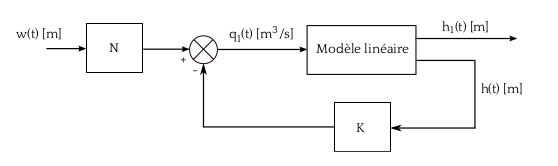
\includegraphics[scale=0.7]{fig2.png}
\captionof{figure}{\textit{ Retour d’état.\cite{ref1}}}
\label{fig2} 
\end{center}


